\documentclass[12pt]{article}       % 設定文件類型為 article,字體大小為 12pt
\usepackage[T1]{fontenc}            % 設定 T1 字型編碼,確保特殊字元的正確顯示
\usepackage{lmodern}                % 強制使用 Latin Modern 字型,提高可讀性和相容性
\usepackage{fontspec}               % 允許使用 OpenType 和 TrueType 字型
\usepackage{graphicx}               % 支援插入圖片
\usepackage{amsmath}                % 提供數學環境和公式支持
\usepackage{csquotes}               % 提供引用格式支援
\usepackage{comment}                % 提供多行註解
\usepackage{ragged2e}
\usepackage{float}
\usepackage{diagbox}  % 加入這行來載入 diagbox 套件
\usepackage{booktabs} % 專業表格格式
\usepackage{siunitx}  % 數值對齊
\usepackage{pgfgantt}



%biber Proposal

%=================================================={{{參考文獻設定}}}==================================================

\usepackage[style=ieee, maxnames=99]{biblatex}          % 設定參考文獻格式為 IEEE,最多顯示 99 個作者
\addbibresource{Proposal.bib}                       % 添加參考文獻檔案 references.bib
\renewcommand{\bibfont}{\fontspec{Times New Roman}}     % 設定參考文獻字體為 Times New Roman
\renewcommand{\UrlFont}{\fontspec{Times New Roman}}     % 設定 URL 連結字體為 Times New Roman
\DeclareFieldFormat{url}{\url{#1}}                      % 格式化 URL                          % 引用你的 .bib 文件

%=================================================={{{目錄設定}}}==================================================

\usepackage{tocloft} % 自訂目錄格式

% 設定目錄的點線填充樣式
\renewcommand{\cftsecleader}{\cftdotfill{\cftdotsep}}           % 章節(section)
\renewcommand{\cftsubsecleader}{\cftdotfill{\cftdotsep}}        % 小節(subsection)
\renewcommand{\cftsubsubsecleader}{\cftdotfill{\cftdotsep}}     % 子小節(subsubsection)

% 設定圖目錄與表目錄的點線
\renewcommand{\cftdotsep}{1}  % 設定點的間距,使其在所有目錄(含圖、表)中都有效

% 設定目錄標題格式,使目錄、圖目錄、表目錄標題一致
\renewcommand{\contentsname}{\centering \LARGE \textbf{目錄}}    % 目錄標題置中,加粗
\renewcommand{\listfigurename}{\centering \LARGE \textbf{圖目錄}} % 圖目錄標題置中,加粗
\renewcommand{\listtablename}{\centering \LARGE \textbf{表目錄}} % 表目錄標題置中,加粗


%=================================================={{{字體設定}}}==================================================

% 設定英文字體
\newfontface\englishfont{Times New Roman}               % 自訂英文字體命令 \englishfont,使用 Times New Roman

\setmainfont[
    ItalicFont={Times New Roman Italic},                % 設定斜體
    BoldFont={Times New Roman Bold},                    % 設定粗體
    BoldItalicFont={Times New Roman Bold Italic}        % 設定粗斜體
]{Times New Roman}                                      % 設定主要英文字體為 Times New Roman

% 設定中文字體

\usepackage{xeCJK}                                      % 使用 xeCJK 宏包以支援中文
\renewcommand{\figurename}{圖}                           % 設定圖表名稱
\renewcommand{\tablename}{表}                            % 修改表格標題為「表」
\setCJKmonofont{標楷體-繁}
\setCJKmainfont[BoldFont={標楷體-繁}, ItalicFont={標楷體-繁}] {標楷體-繁}
%=================================================={{{版面設定}}}==================================================

% 設定頁面邊界,適用 A4 紙張
\usepackage[top=2cm, bottom=2cm, left=2cm, right=2cm, a4paper]{geometry}

% 設定行距與段落格式
\usepackage{setspace}
\onehalfspacing % 設定 1.5 倍行距
\setlength{\parskip}{6pt} % 設定段落間距 6pt
\setlength{\parindent}{2em} % 設定段落首行縮排 2 個字元

%=============================================================================================================================
%=============================================================================================================================
%=============================================================================================================================

\begin{document}
%=================================================={{{封面}}}==================================================
\begin{titlepage}
    \centering
    \vspace*{1cm} % 增加上方間距

    {\LARGE \textbf{元智大學工程學院機械工程學系}} \\[0.5cm] % 標題較大且加粗
    {\LARGE {Department of Mechanical Engineering}} \\[0.5cm] % 標題較大且加粗
    {\LARGE {College of Engineering}} \\[0.5cm]
    {\LARGE {Yuan Ze University}}

    \vfill % 這一行讓前面的資訊靠上排列

    {\LARGE{機電整合期末專題企劃書}} % 這行會上下左右完全置中

    \vfill % 這一行讓後面的資訊靠下排列

    {\LARGE {1100826 王子晨}}\\[6cm]
    {\LARGE {指導教授:吳昌暉\hspace{0.5cm}博士}}\\[0.5cm]

\end{titlepage}
\newpage
%=================================================={{{封面}}}==================================================

\pagenumbering{roman}  
\setcounter{page}{1}  % 從 I 開始

%=================================================={{{中文摘要}}}==================================================

\section*{\centering 摘要}  % 只讓標題置中
\addcontentsline{toc}{section}{摘要}  % 手動加入摘要到目錄

%==============================摘要內容==============================

\hspace{2em}本研究旨在設計一款基於影像處理技術的循線自走車,透過攝影機捕捉地面標線影像並使用影像處理算法進行自動識別,實現車輛自動跟隨標線行駛。
車輛運用了麥克納姆輪系統,具備多向移動能力,提供更高的靈活性與操作精度。在車輛運行過程中,攝影機會即時捕捉前方及周圍的環境影像,通過影像處理技術進行辨識,判斷標線位置及車輛偏差,並依此進行位置與方向的調整,確保車輛沿標線精確行駛。
研究中選用了OV2640攝影鏡頭作為感測器,並搭配TT馬達和Arduino控制器進行運動控制。車輛的運行指令由個人電腦進行計算,並利用Wi-Fi進行車輛與控制器之間的通訊。預處理部分將利用透視變換、灰階處理、高斯模糊等技術來處理影像,為後續的車道偵測與控制算法提供準確的數據支持。

%==============================摘要內容==============================
\newpage  % 插入換頁命令,將目錄和後續內容分開


%=================================================={{{目錄}}}==================================================

\begin{center}
    \tableofcontents    % 生成目錄
%========================={{{可有可無}}}=========================
\newpage 

\addtocontents{toc}{\protect\setcounter{tocdepth}{0}} % 暫時關閉目錄深度,讓圖目錄不顯示在目錄中
\listoffigures      % 生成圖目錄
\addtocontents{toc}{\protect\setcounter{tocdepth}{2}} % 恢復目錄深度(如果你的章節結構需要更深層級,請調整數值)
%\newpage  
\listoftables       % 生成表目錄

%========================={{{可有可無}}}=========================
\end{center} 

%=================================================={{{內容開始}}}==================================================
\newpage  % 插入換頁命令,將目錄和後續內容分開
\pagenumbering{arabic}  % 開始使用阿拉伯數字頁碼
\setcounter{page}{1}  % 設定頁碼從 1 開始

%\englishfont{this is an example of mixed English and Chinese.}

\section{\centering 整體功能}
%==============================內文==============================
\hspace{2em}本期末專題旨在設計一款基於影像處理技術的循線自走車。
車輛將利用攝影機捕捉地面標線影像,並通過影像處理算法實現自動跟隨標線行駛。
專題將融合麥克納姆輪系統,讓車輛能夠實現多向移動,提供更高的靈活性和操作精度。

在車輛運行過程中,攝影機將即時捕捉前方及周圍的環境影像,並利用影像處理技術進行辨識,判斷標線位置和車輛的當前偏差。車輛將根據這些信息,進行位置與方向調整,從而自動修正其行駛路徑,確保沿著標線精確行駛。

此外,通過麥克納姆輪的設計,車輛將具備前進、後退、左右側向移動以及旋轉等多種運動模式,這使得車輛在複雜路徑中具有更高的操作靈活性。

\section{\centering 機械結構草圖}

%==============================內文==============================
\hspace{2em}機械結構草圖與使用之麥克納姆輪如下:

\begin{figure}[H]
    \centering
    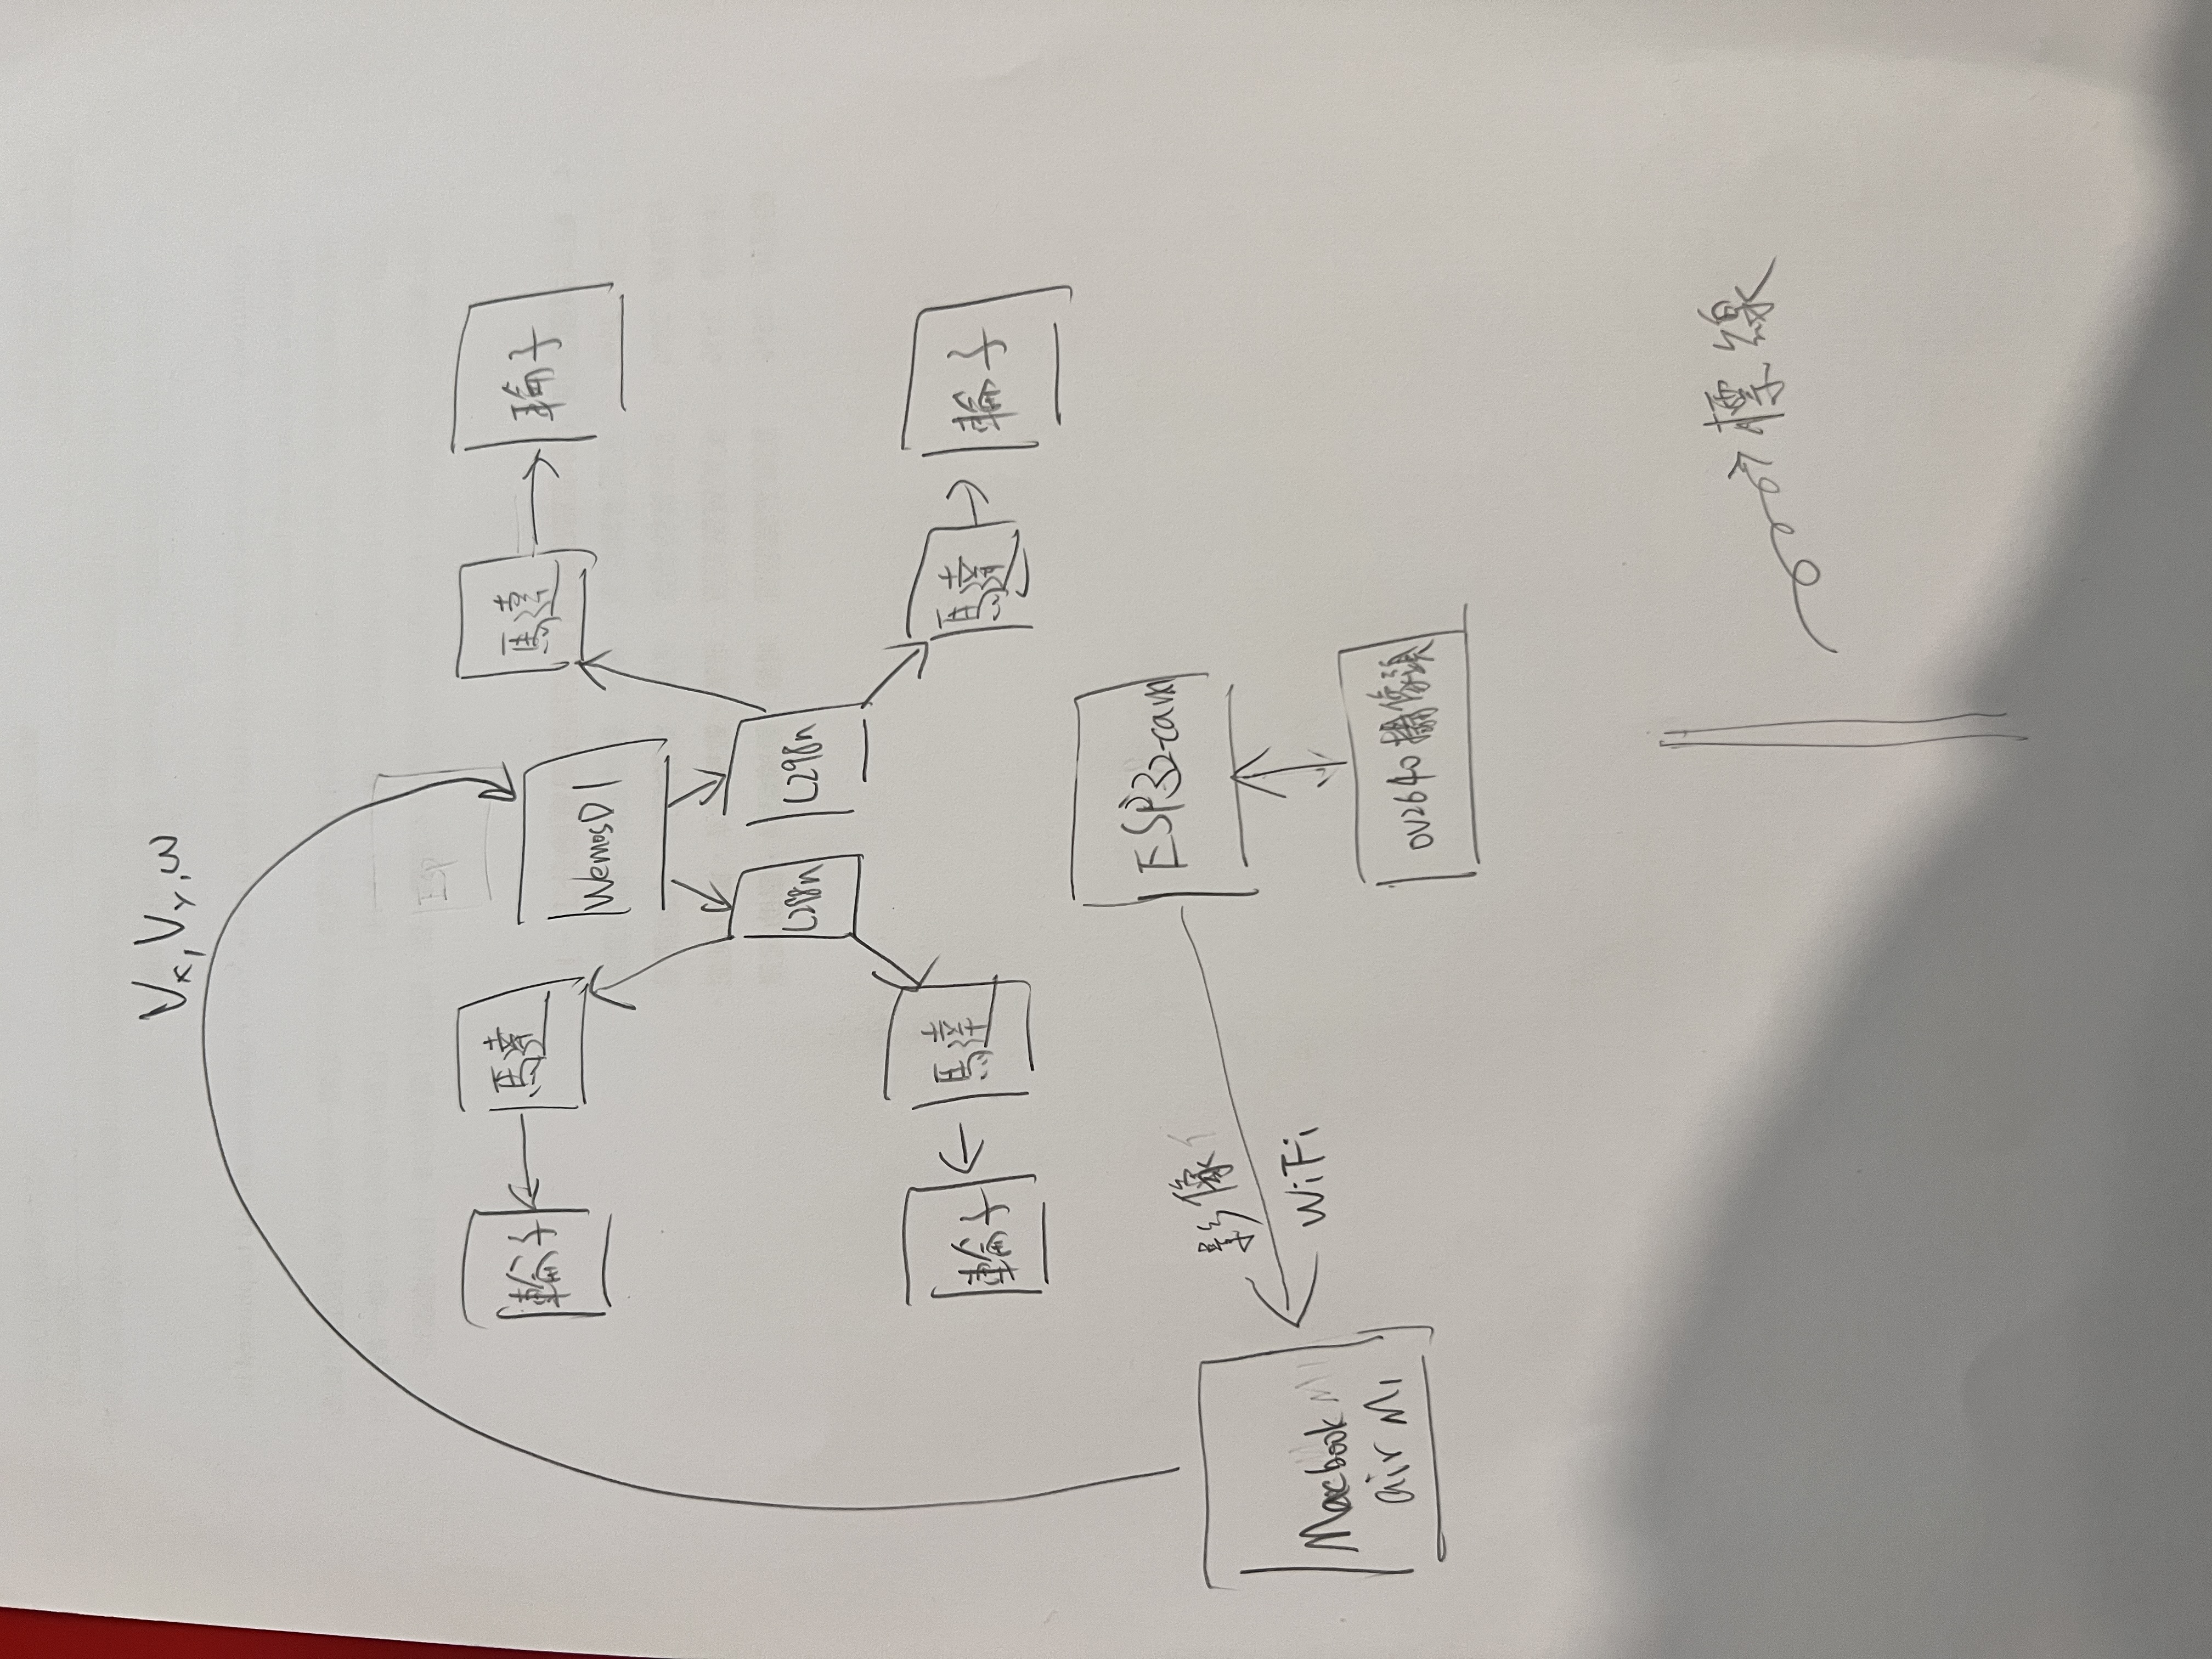
\includegraphics[width=0.8\textwidth, angle=270]{IMG_5917.jpg}     %圖片檔案名稱
    \caption{機械結構草圖}    %圖片檔案名稱
    \label{fig:IMG_5917}    %為圖片添加標籤
    %如\ref{fig:MxzONoG}所示
\end{figure}

\begin{figure}[H]
    \centering
    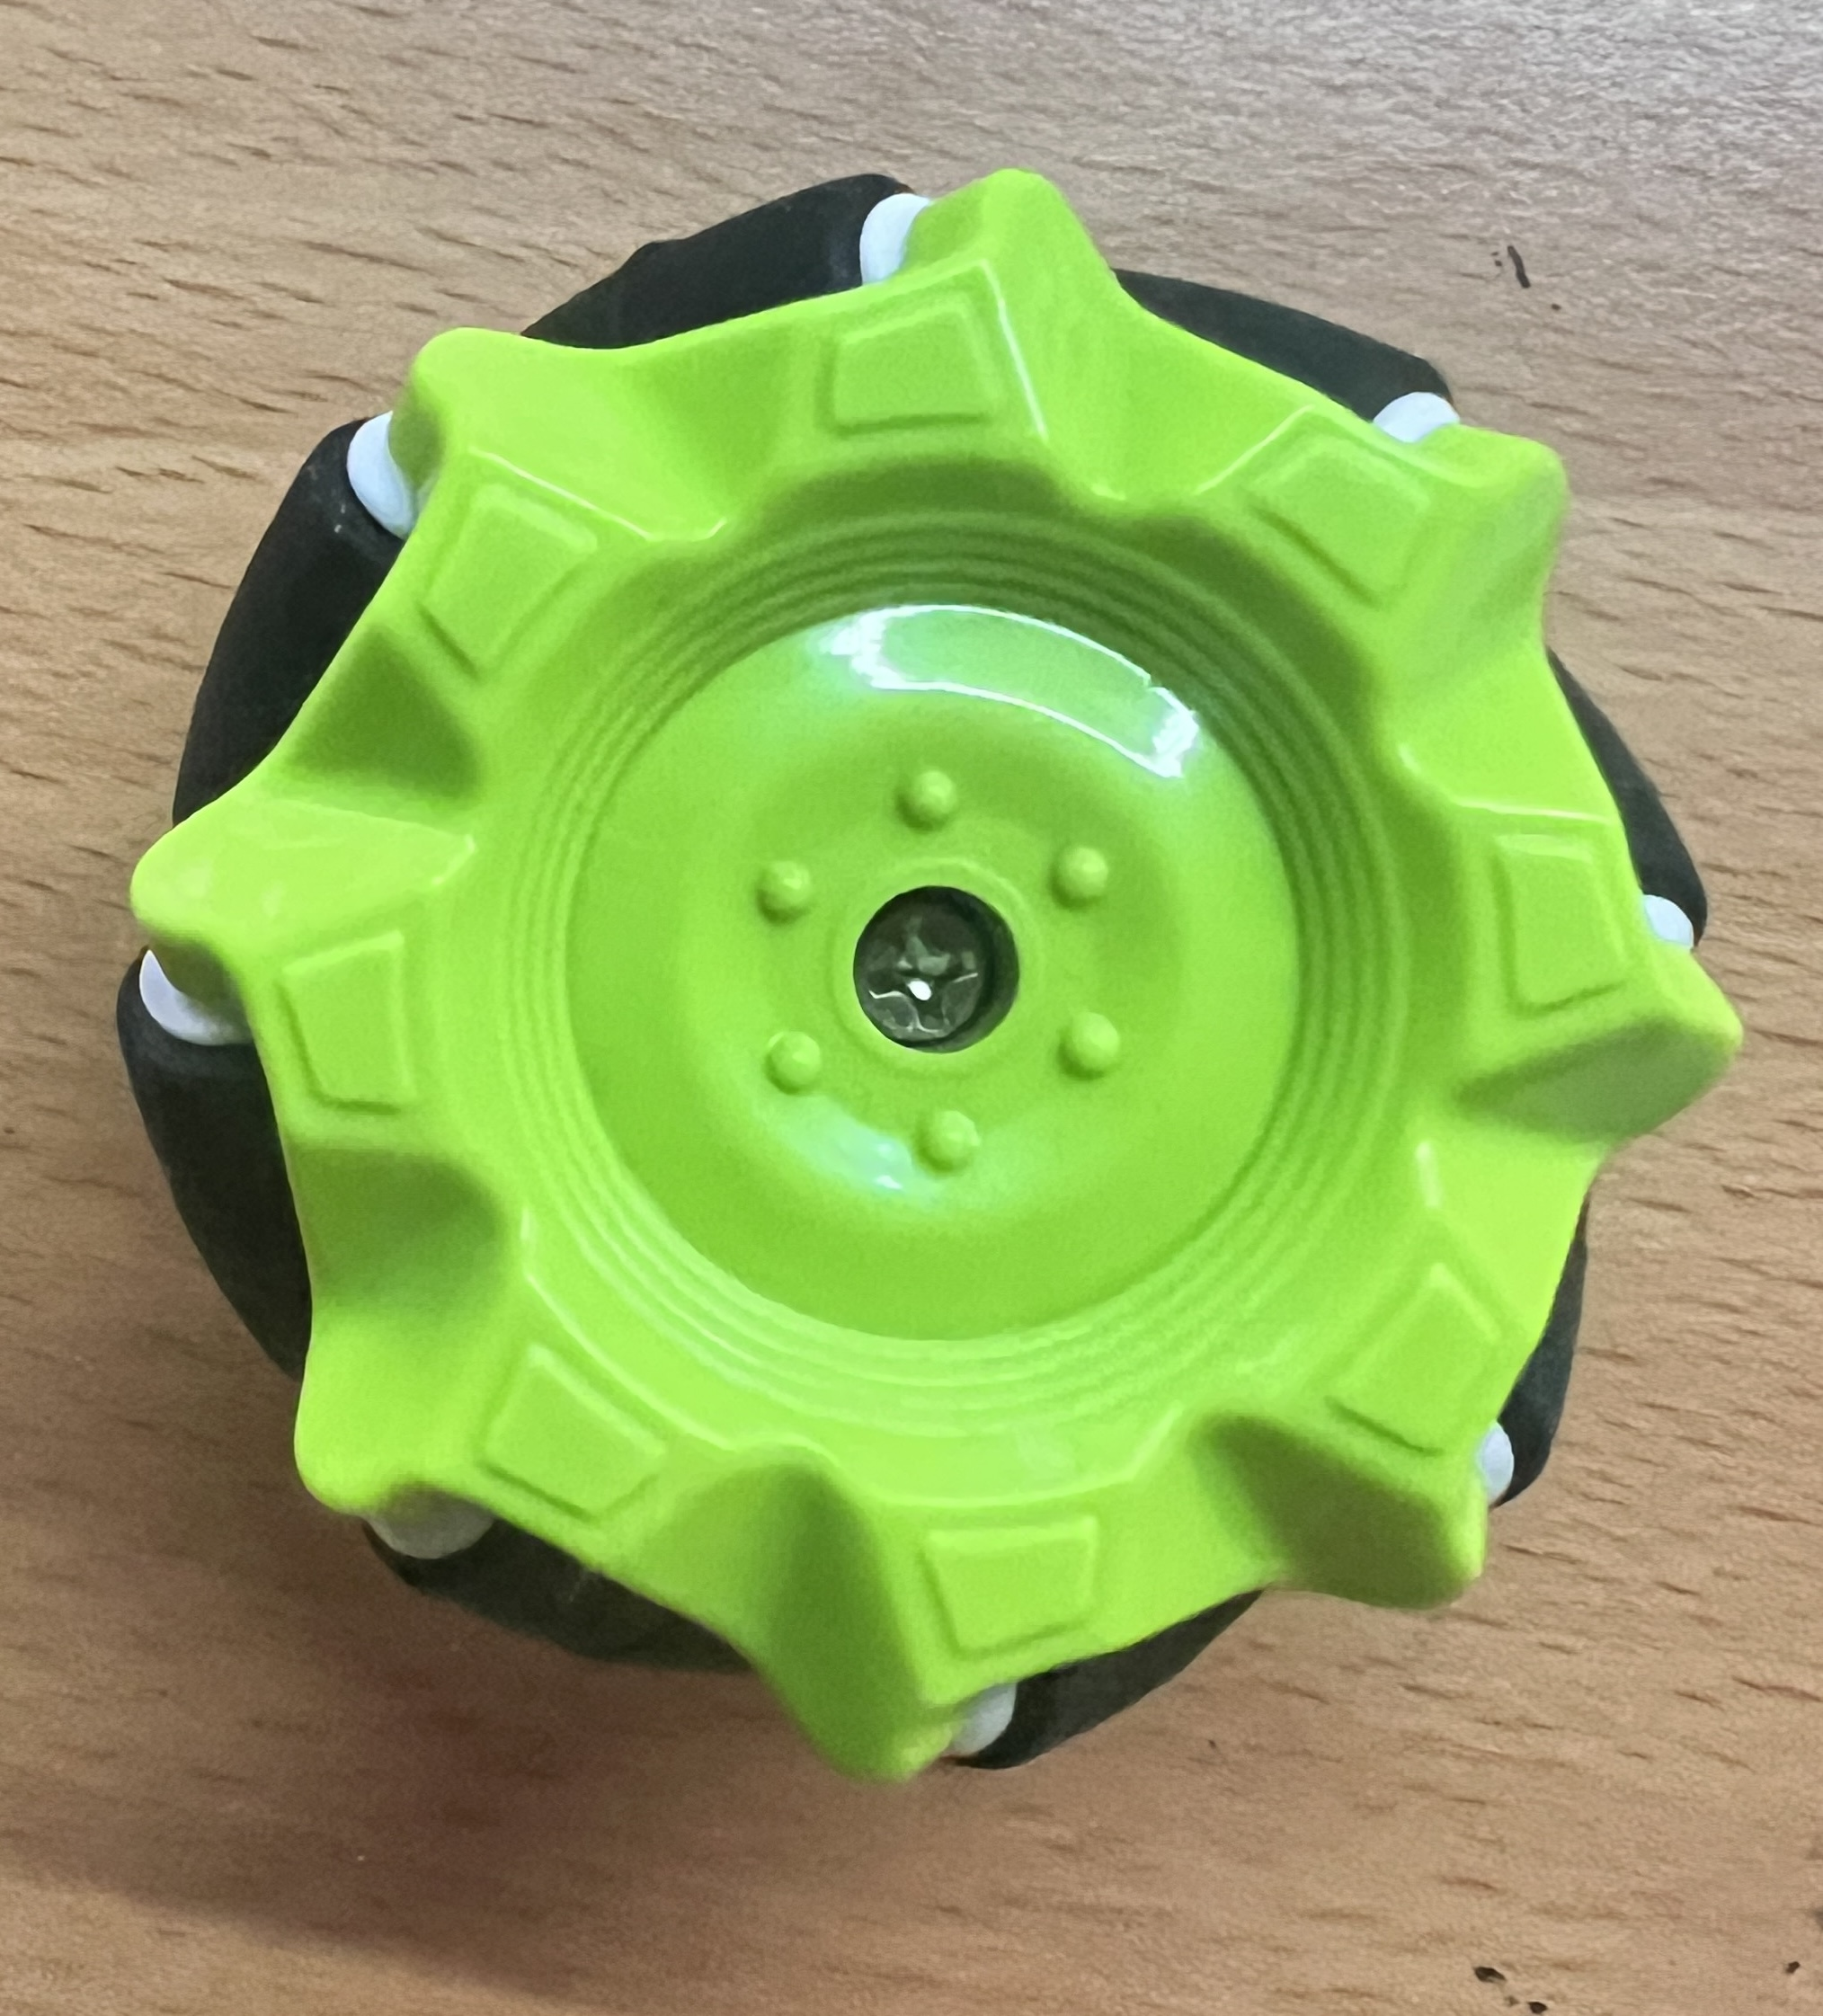
\includegraphics[width=0.7\textwidth]{IMG_5906.jpg}     %圖片檔案名稱
    \caption{麥克納姆輪(直徑58mm)}    %圖片檔案名稱
    \label{fig:IMG_5906}    %為圖片添加標籤
    %如\ref{fig:MxzONoG}所示
\end{figure}

%==============================內文==============================

\section{\centering 致動器的功能與數目列表}


%==============================內文==============================
\hspace{2em}採用TT馬達來驅動車輛,使其具備靈活的多向運動能力。下表是功能與數量(如表\ref{tab:TT2}所示)和規格表(如表\ref{tab:ttm}所示):

\begin{table}[H]
    \centering
    \caption{致動器的功能與數目列表}
    \vspace{6pt} % 增加空格
    \label{tab:TT2}
    \begin{tabular}{lll}
        \toprule
        \textbf{項目} & \textbf{功能} & \textbf{數量}\\
        \midrule
        TT減速馬達  & 每個麥克納姆輪提供獨立的驅動 &4\\
        \bottomrule
    \end{tabular}
    %如\ref{tab:TT2}所示
\end{table}

\begin{table}[H]
    \centering
    \caption{TT 馬達規格\cite{JustMakeIt_TT_Motor}}
    \vspace{6pt} % 增加空格
    \label{tab:ttm}
    \begin{tabular}{ll}
        \toprule
        \textbf{項目} & \textbf{規格} \\
        \midrule
        減速比  & 1:48 \\
        工作電壓  & 6V \\
        空載電流 & $\leq$ 240 $\text{mA}$ \\
        空載轉速  & 270 $\pm$10$\%$ RPM \\
        扭矩  & 1.5 $\text{kgf} \cdot \text{cm}$ \\
        \bottomrule
    \end{tabular}
\end{table}

\begin{figure}[H]
    \centering
    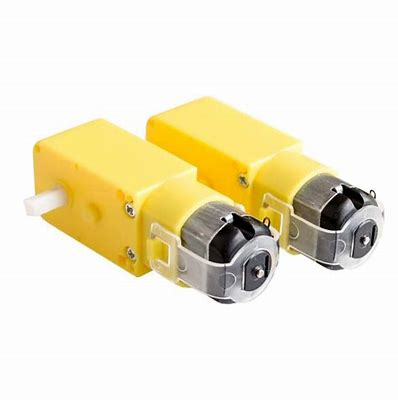
\includegraphics[width=0.7\textwidth]{MxzONoG.png}     %圖片檔案名稱
    \caption{TT 馬達\cite{JustMakeIt_TT_Motor}}    %圖片檔案名稱
    \label{fig:MxzONoG}    %為圖片添加標籤
    %如\ref{fig:MxzONoG}所示
\end{figure}

%==============================內文==============================

\section{\centering 感測器的功能與數目列表}

%==============================內文==============================
\hspace{2em}感測器部分將選用 OV2640 攝影鏡頭。以下是關於 OV2640 的功能與數目列表:
\begin{table}[H]
    \centering
    \caption{感測器的功能與數目列表}
    \vspace{6pt} % 增加空格
    \label{tab:OV26401}
    \begin{tabular}{lll}
        \toprule
        \textbf{項目} & \textbf{功能} & \textbf{數量}\\
        \midrule
        OV2640 攝影鏡頭  & 拍攝影像 &1\\
        \bottomrule
    \end{tabular}
    %如\ref{tab:TT2}所示
\end{table}

\begin{table}[H]
    \centering
    \caption{OV2640 攝影鏡頭規格\cite{taiwansensor_OV2640}}
    \vspace{6pt} % 增加空格
    \label{tab:OV2640_Specs}
    \begin{tabular}{ll}
        \toprule
        \textbf{項目} & \textbf{規格} \\
        \midrule
        感測器類型 & 1/4 吋 CMOS \\
        解析度 & 1600$\times$1200 \\
        幀率  & 15fps \\
        水平視角 & 63$^\circ$ \\
        垂直視角  & 47$^\circ$ \\
        \bottomrule
    \end{tabular}
\end{table}

%==============================內文==============================

\section{\centering 控制器的功能與數目列表}

%==============================內文==============================
\hspace{2em}控制器的部分預計使用兩塊Arduino板子與一台個人電腦、搭配l298n進行控制。功能與數目列表如下表(表\ref{tab:c}、\ref{tab:Wemos}、\ref{tab:macbook_m1})所示。
三台電腦間利用Wi-Fi進行通訊。

\begin{table}[H]
    \centering
    \caption{致動器的功能與數目列表}
    \vspace{6pt} % 增加空格
    \label{tab:c}
    \begin{tabular}{lll}
        \toprule
        \textbf{項目} & \textbf{功能} & \textbf{數量}\\
        \midrule
        Wemos D1  & 接收個人電腦指令控制l298n &1\\
        ESP32-CAM  & 拍攝影像並傳輸至個人電腦 &1\\
        MacBook M1  & 影像偵測與控制演算法計算 &1\\
        l298n  & 麥克納姆輪 &2\\
        \bottomrule
    \end{tabular}
    %如\ref{tab:TT2}所示
\end{table}

\begin{table}[H]
    \centering
    \caption{控制器規格表\cite{taiwaniot_WemosD1}\cite{ESP32CAM}}
    \vspace{6pt} % 增加空格
    \label{tab:Wemos}
    \begin{tabular}{lll}
        \toprule
        \textbf{項目} & \textbf{Wemos D1} & \textbf{ESP32-CAM }\\
        \midrule
        處理器 & ESP8266 &ESP32\\
        記憶體 & 4MB  &4MB\\
        無線連接 & 802.11 b/g/n Wi-Fi& 802.11 b/g/n Wi-Fi\\
        I/O 引腳 & 11 &9\\
        電源 & 5V &5V\\
        \bottomrule
    \end{tabular}
\end{table}

\begin{table}[H]
    \centering
    \caption{MacBook Air M1 與比較機種規格}
    \vspace{6pt} % 增加空格
    \label{tab:macbook_m1}
    \begin{tabular}{ll}
        \toprule
        \textbf{元件} & \textbf{MacBook Air M1} \\
        \midrule
        處理器 (CPU)  & Apple M1 (8 核心)  \\
        記憶體 (RAM)  & 8GB Unified Memory  \\
        硬碟 (Storage) & 256GB SSD  \\
        顯示卡 (GPU)  & Apple M1 內建 GPU (7 核心)  \\
        作業系統 (OS)  & macOS Sequoia \\
        電池容量 (Battery) & 49.9Wh \\
        \bottomrule
    \end{tabular}
\end{table}

%==============================內文==============================

\section{\centering 演算法設計}
%==============================內文==============================
\hspace{2em}演算法的設計包括三個部分,分別是預處理、偵測、控制,運算全都由個人電腦(MacBook Air M1)進行運算。

%==============================內文==============================

\subsection{預處理} 
%==============================內文==============================
\hspace{2em}預處理部分包括透視變換、灰階處理、高斯模糊、二值化、Canny邊緣偵測,將接收到的影像進行處理,提供後續偵測使用。

%==============================內文==============================

\subsubsection{透視變換}
%==============================內文==============================
\hspace{2em}首先,對捕獲的影像進行透視變換,將影像轉換為以車輛為原點的二維座標系統,這樣有助於確定車輛與道路的相對位置,並為後續的計算提供準確的基準。

本專題將利用鏡頭往斜下的角度拍攝。採用逆透視變換(Inverse Perspective Mapping,IPM)\cite{lin_2001}\cite{bertozz1998stereo}\cite{mallot1991inverse}技術處理影像,可以將像素座標轉換為地面座標,取得影像中精確的距離。
技術處理影像,可以將像素座標轉換為地面座標,取得影像中精確的距離。
透視變換的核心在於去除透視效應,以便將影像中的道路線條轉換為平行的直線。這樣的變換有助於車輛識別路徑,使後續演算法能夠更容易地進行路徑規劃與車道偵測。

首先將影像像素座標系$(u,v)$轉換為圖像座標系$(x,y)$。
加入相機的水平視角$HFOV$與相機的垂直視角$VFOV$、相機俯仰角$\theta_{c}$,將圖像座標轉換為相機座標$(x_{c},y_{c},z_{c})$。
接著將相機座標系轉換為車輛標系$(x_w,y_w,z_w)$,以取得拍攝影像中內容物與車輛之相對位置。流程圖如下:
\begin{figure}[H]
    \centering
    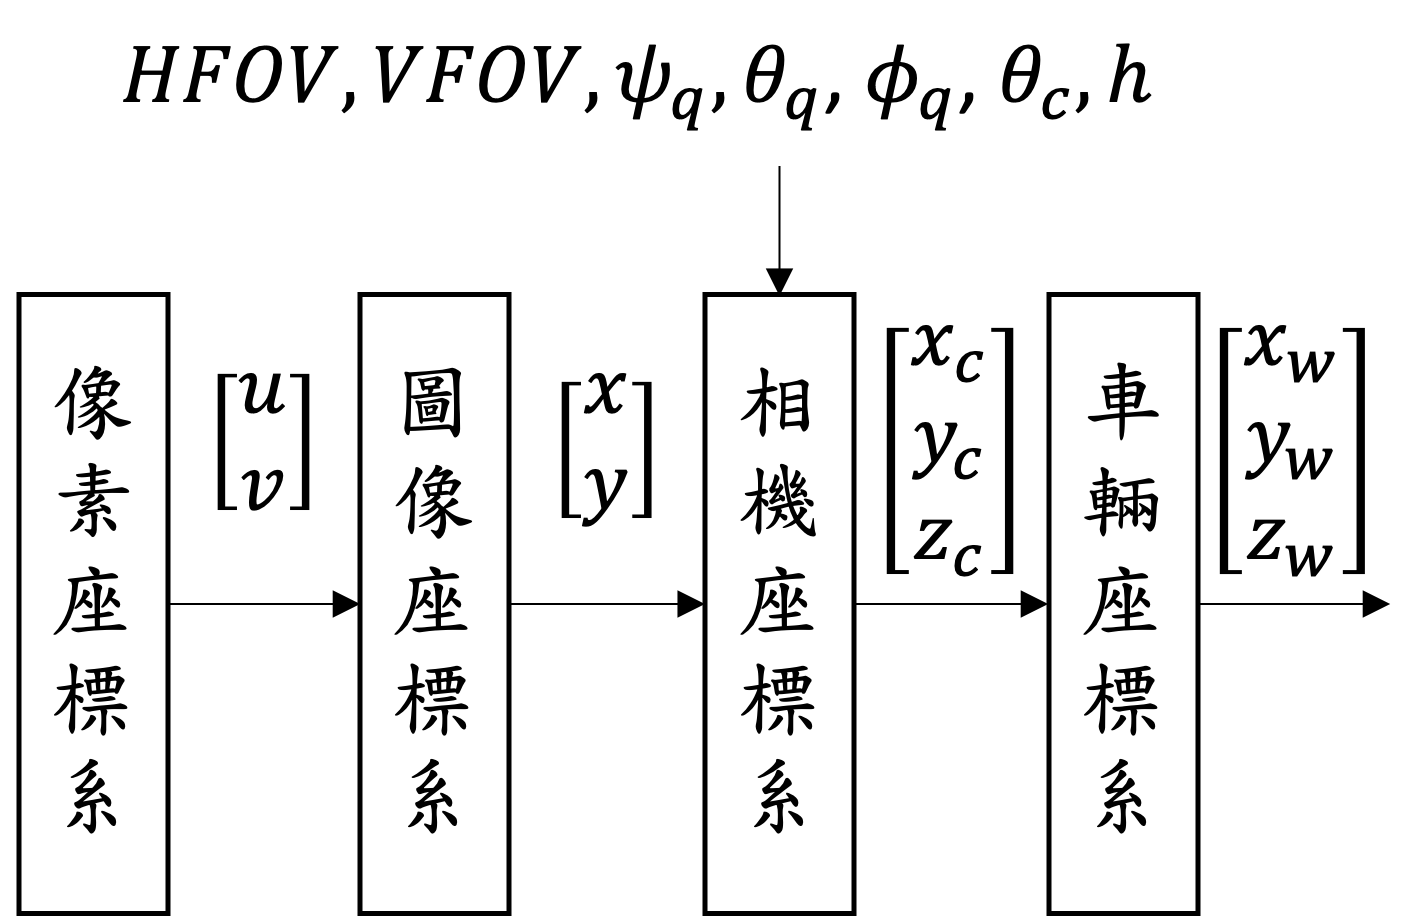
\includegraphics[width=0.7\textwidth]{123.png}     %圖片檔案名稱
    \caption{透視變換流程圖}    %圖片檔案名稱
    \label{fig:123}    %為圖片添加標籤
    %如\ref{fig:MxzONoG}所示
\end{figure}
將像素座標轉換為無人機相對於地平面的世界座標時,過程涉及相機的內參矩陣$K$、旋轉矩陣$R$以及相機高度$h$。要算相機的內參矩陣首先需得出影像的水平焦距$f_{x}$、影像的垂直焦距$f_{y}$和影像的中心座標$(c_x,c_y)$。

影像的水平焦距$f_{x}$公式如式(\ref{eq:fx}),W為影像的寬度,HFOV為相機的水平視角。
影像的垂直焦距$f_{y}$公式如式(\ref{eq:fy}),H為影像的寬度,VFOV為相機的垂直視角。
\begin{align}
    f_{x}=\frac{W}{2\cdot\tan\left(\frac{HFOV}{2}\right)}
    \label{eq:fx}
    \\
    f_{y}=\frac{H}{2\cdot\tan\left(\frac{VFOV}{2}\right)}
    \label{eq:fy}
\end{align}

影像的中心座標$(c_x,c_y)$公式如式(\ref{eq:cx})、式(\ref{eq:cy}):
\begin{align}
    c_{x}=\frac{W}{2}
    \label{eq:cx}
    \\
    c_{y}=\frac{H}{2}
    \label{eq:cy}
\end{align}

式(\ref{eq:k})為相機內參矩陣K。
\begin{align}
    K &=
    \begin{bmatrix}
        f_{x}       & 0             & c_{x}     \\
        0           & f_{y}         & c_{y}     \\
        0           & 0             & 1
    \end{bmatrix} 
    \label{eq:k}
\end{align}

旋轉矩陣R用來表示相機相對於世界座標系的旋轉。
此處忽略車輛進行中的晃動。旋轉矩陣R如下:
\begin{align}
    R=&
    \begin{bmatrix}
        1   & 0  & 0 \\
        0   & \cos(\theta_{c})   & -\sin(\theta_{c}) \\
        0   & \sin(\theta_{c})   & \cos(\theta_{c}) \\
    \end{bmatrix} 
    \label{eq:R2}
\end{align}

將像素座標系$(x,y)$轉換為圖像座標系的公式如式(\ref{eq:xy1}):
\begin{align}
    \begin{bmatrix}
        x       \\
        y    \\
        1        
    \end{bmatrix} 
     &=K^{-1}\cdot
     \begin{bmatrix}
        u       \\
        v       \\
        1        
    \end{bmatrix} 
    \label{eq:xy1}
\end{align}

將圖像座標系轉換為相機座標系的公式如式(\ref{eq:xcyczc}):
\begin{align}
    \begin{bmatrix}
        x_{c}   \\
        y_{c}   \\
        z_{c}        
    \end{bmatrix} 
     &=R\cdot
     \begin{bmatrix}
        x       \\
        y       \\
        1        
    \end{bmatrix} 
    \label{eq:xcyczc}
\end{align}

實際測試結果如下圖所示。將實際拍攝影像投影至以相機為原點的平面上,即可計算拍攝目標物與車輛之距離。
\begin{figure}[H]
    \centering
    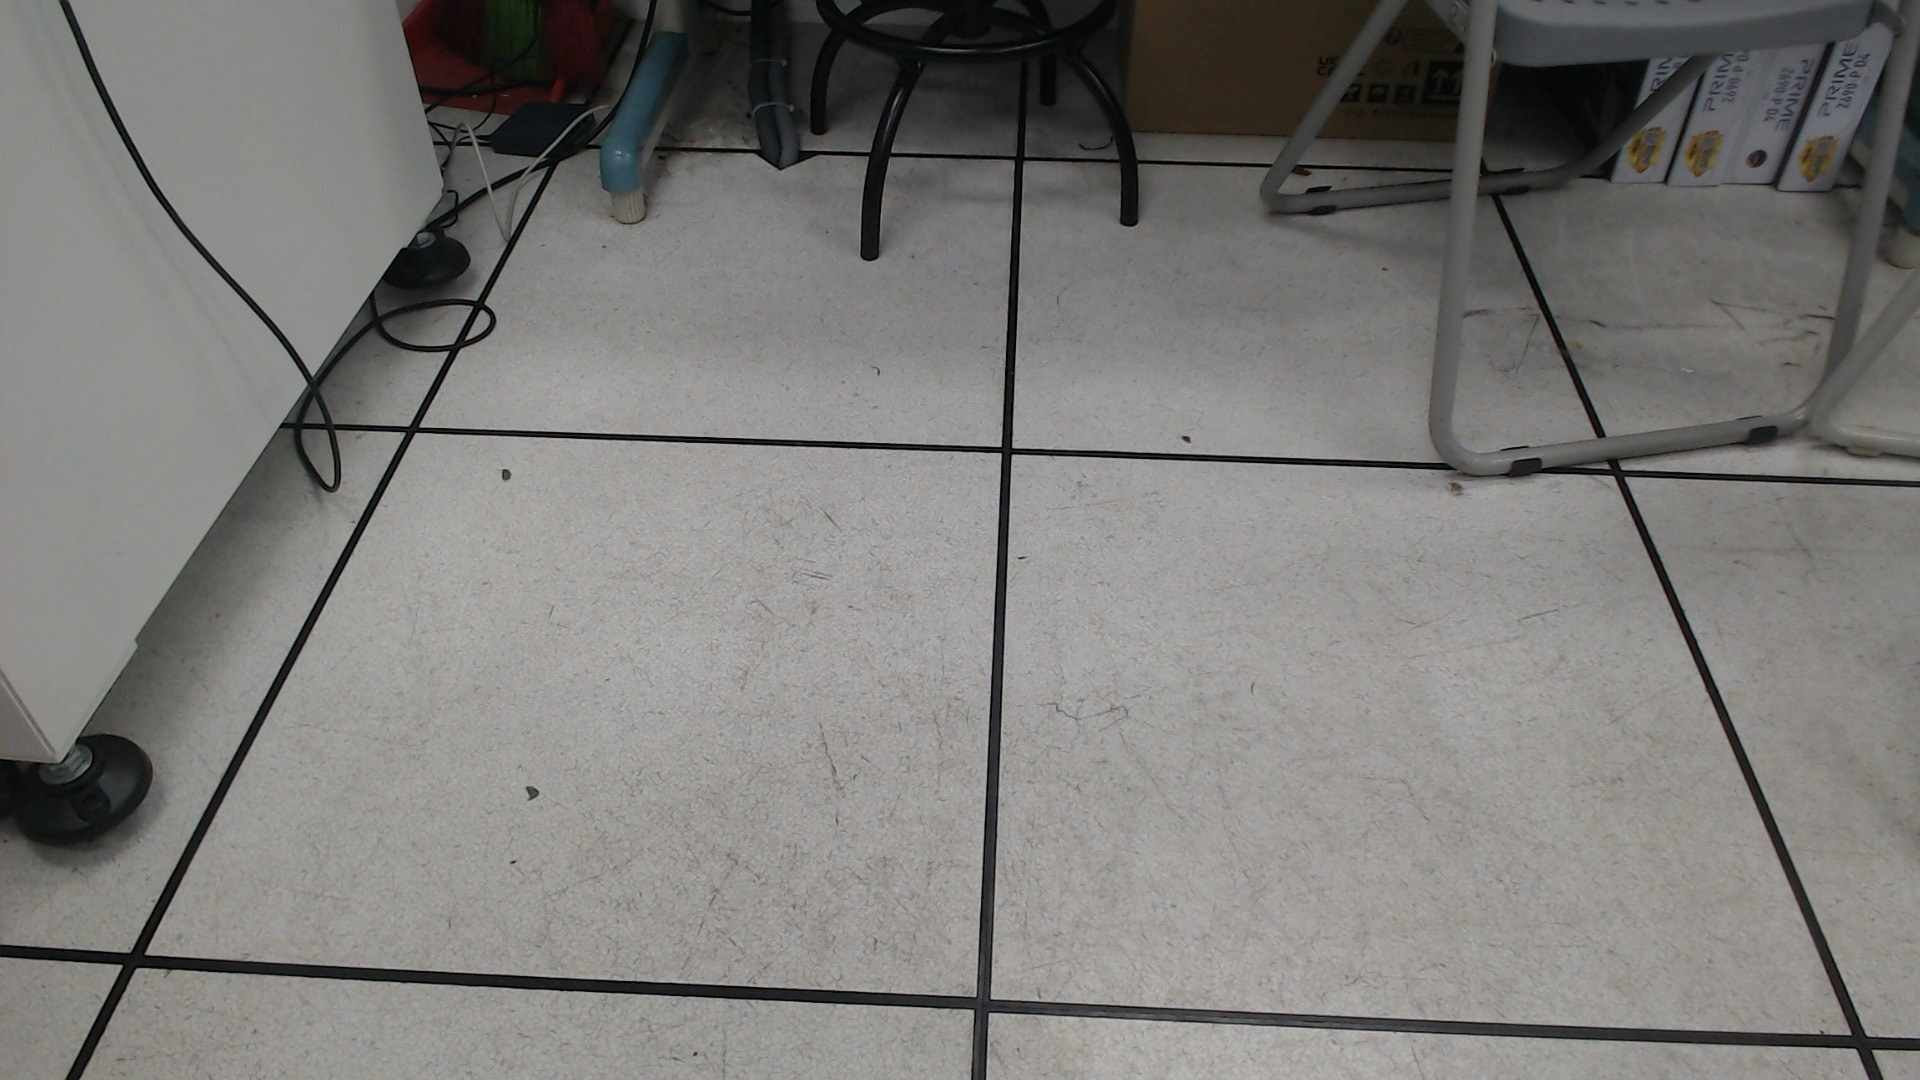
\includegraphics[width=0.7\textwidth]{11.jpg}     %圖片檔案名稱
    \caption{尚未進行透視變換之原始圖片}    %圖片檔案名稱
    \label{fig:11}    %為圖片添加標籤
    %如\ref{fig:MxzONoG}所示
\end{figure}
\begin{figure}[H]
    \centering
    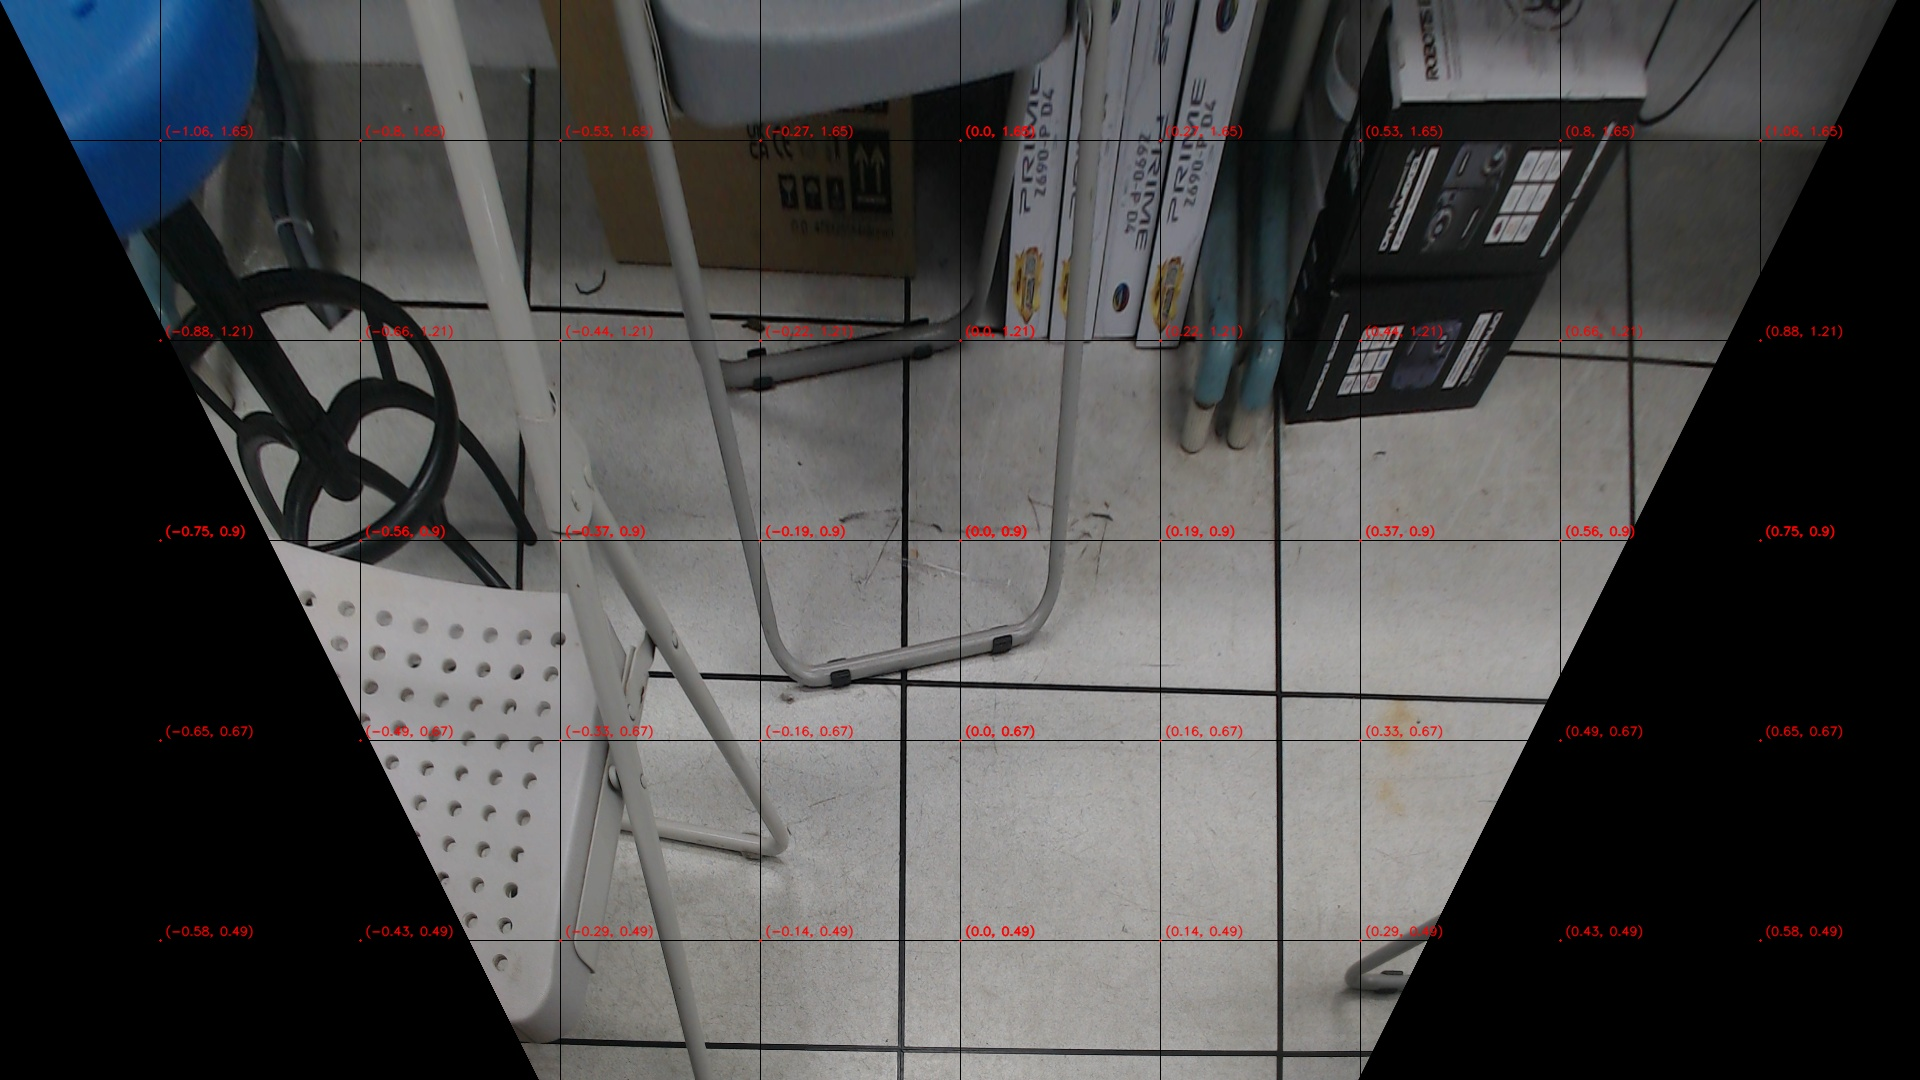
\includegraphics[width=0.7\textwidth]{22.jpg}     %圖片檔案名稱
    \caption{經透視變換後影像}    %圖片檔案名稱
    \label{fig:22}    %為圖片添加標籤
    %如\ref{fig:MxzONoG}所示
\end{figure}

下圖(如圖\ref{fig:frame_with_points_real}所示)與下表(如表\ref{tab:error_comparison}所示)為實際測量之結果,並計算誤差,若參數設置準確,絕對誤差大約為0.7公分左右。

\begin{figure}[H]
    \centering
    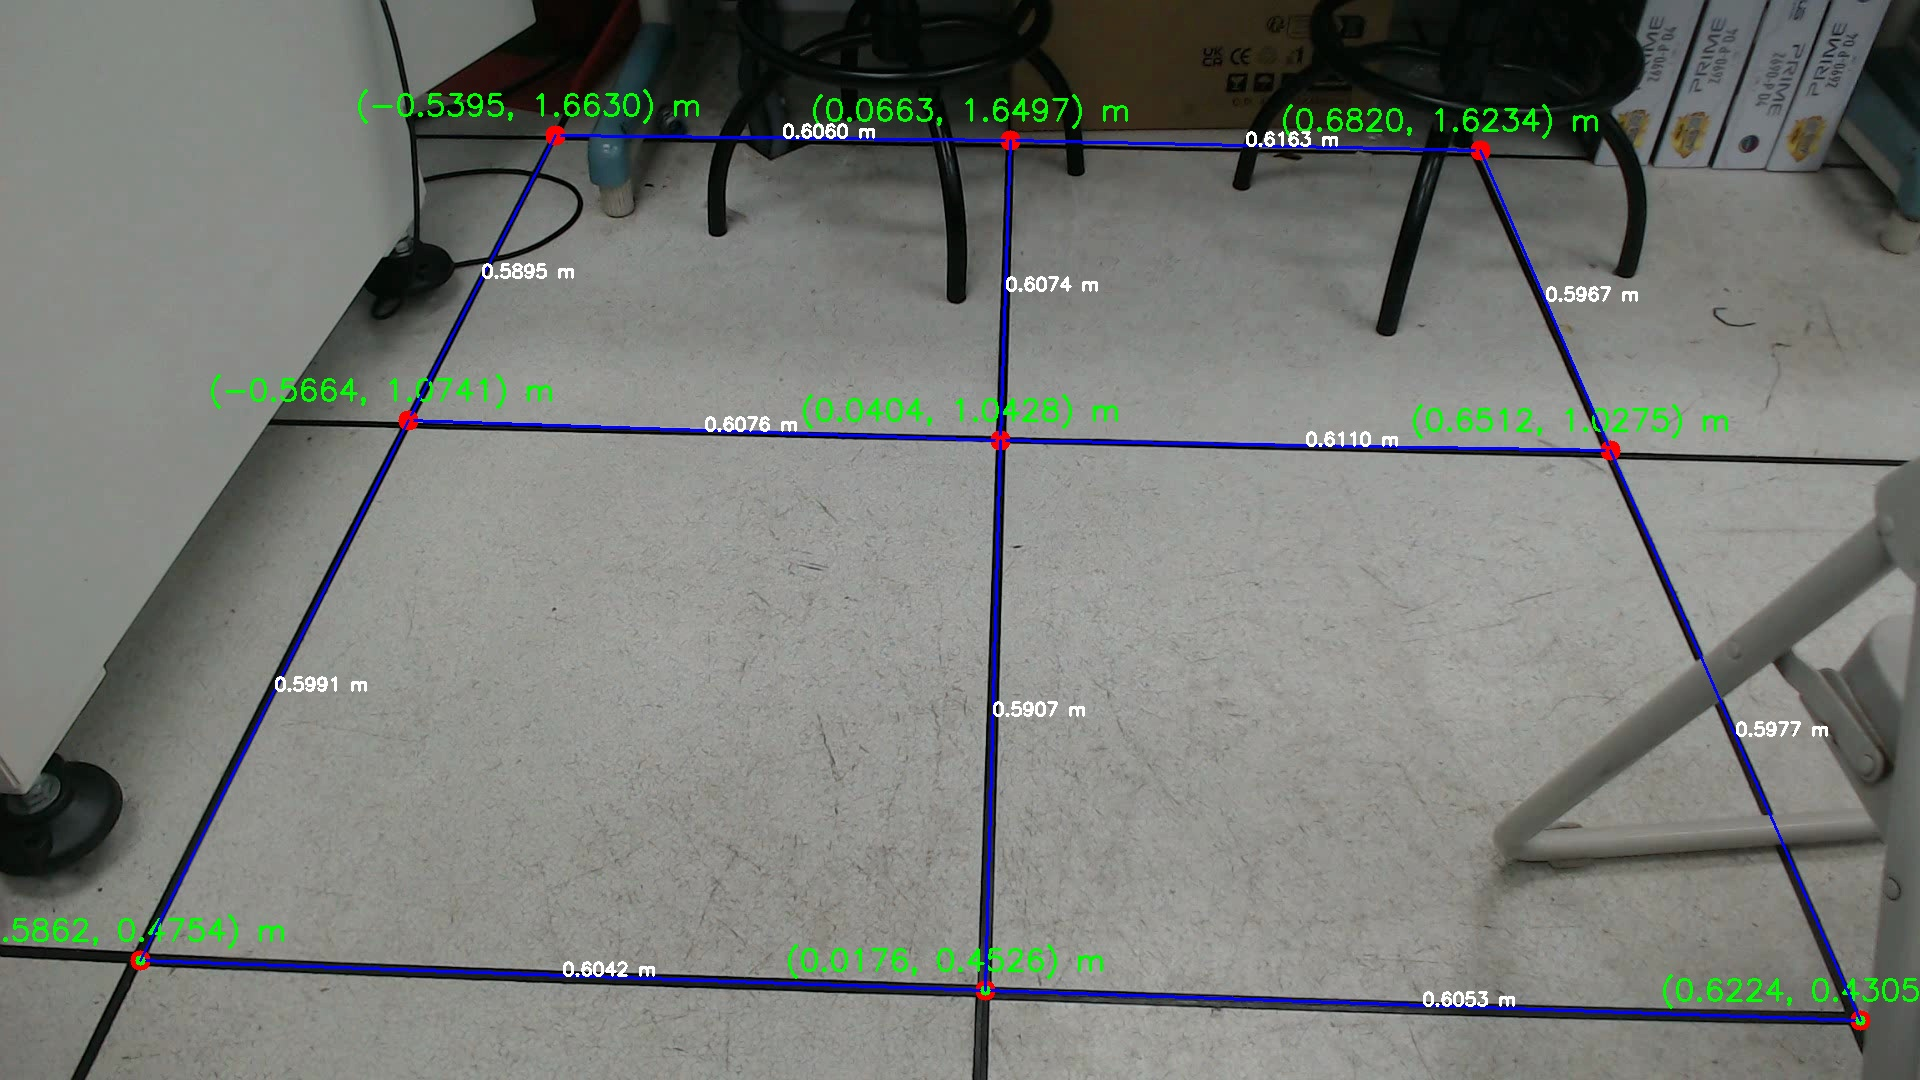
\includegraphics[width=0.7\textwidth]{frame_with_points_real.jpg}     %圖片檔案名稱
    \caption{實際測量地板尺寸}    %圖片檔案名稱
    \label{fig:frame_with_points_real}    %為圖片添加標籤
    %(如圖\ref{fig:frame_with_points_real}所示)
\end{figure}

\begin{table}[H]
    \centering
    \caption{透視變換誤差}
    \vspace{6pt} % 增加空格
    \label{tab:error_comparison}
    \begin{tabular}{lS[table-format=2.2]S[table-format=2.2]}
        \toprule
        MAE(m) & 0.007  \\
        MRE(\%) & 1.168 \\
        \bottomrule
    \end{tabular}
\end{table}
%==============================內文==============================

\subsubsection{灰階處理}
%==============================內文==============================
\hspace{2em}將彩色影像轉換為灰階影像,這樣能有效減少計算量,同時保留影像的基本結構特徵,便於後續處理。
這樣的轉換方式基於人眼對不同顏色敏感度的權重選擇,使得轉換後的影像仍然保持較高的可辨識度。

由行車圖片進行測試,圖\ref{fig:1}為原始圖片,圖\ref{fig:2}為經灰階處理之圖片。
\begin{figure}[H]
    \centering
    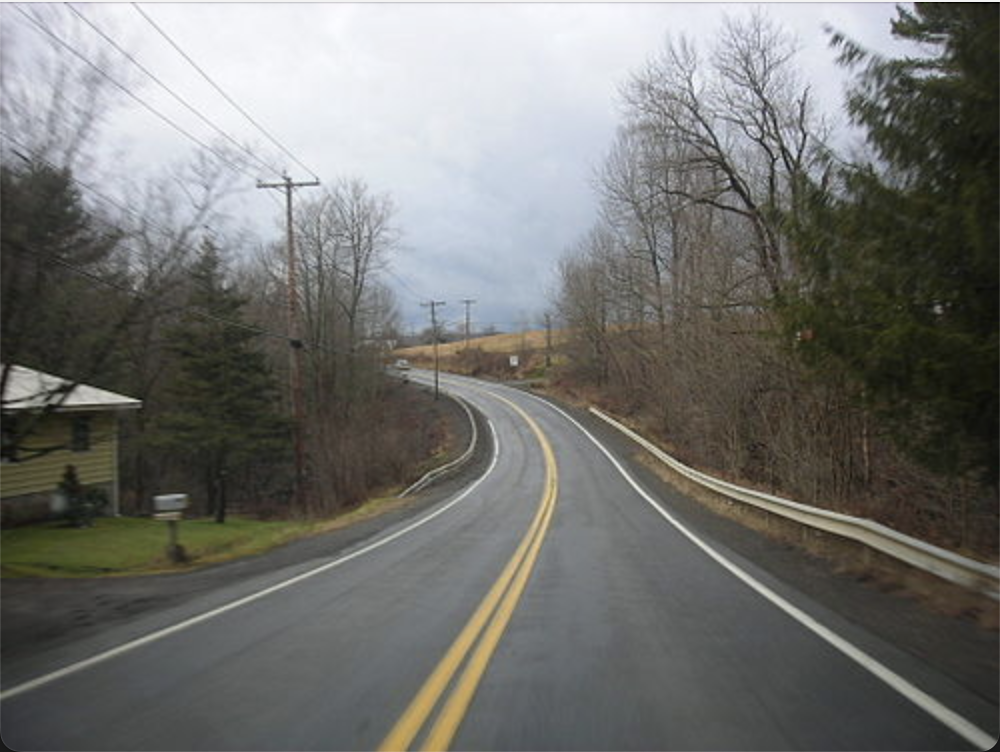
\includegraphics[width=0.7\textwidth]{1.png}     %圖片檔案名稱
    \caption{待測試之原始圖片}    %圖片檔案名稱
    \label{fig:1}    %為圖片添加標籤
    %如\ref{fig:MxzONoG}所示
\end{figure}

\begin{figure}[H]
    \centering
    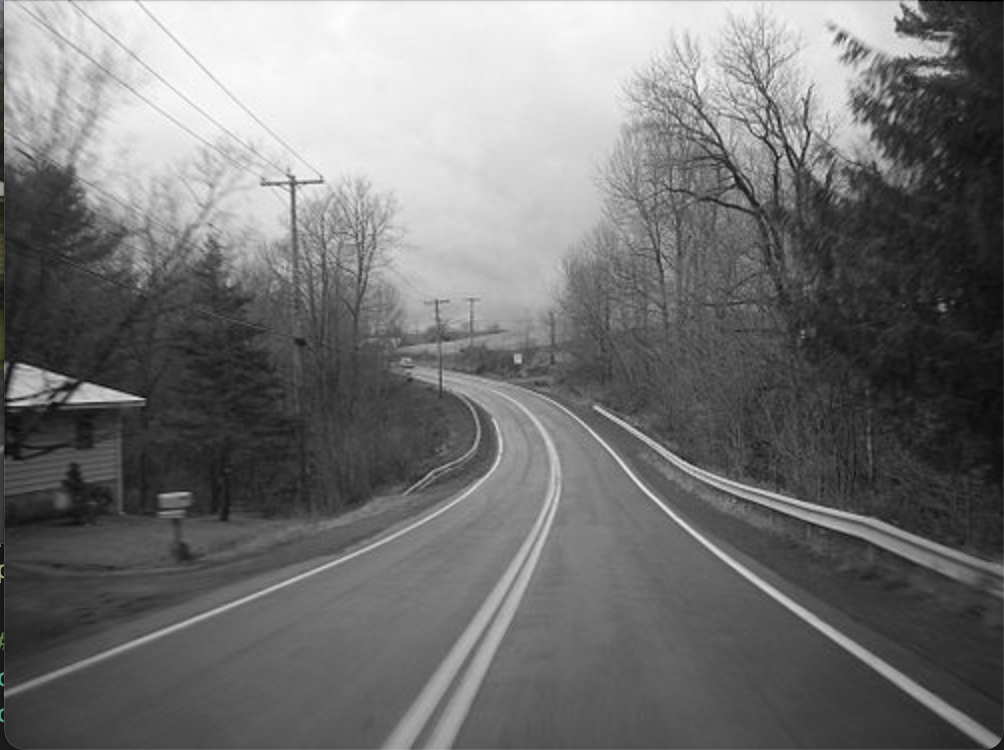
\includegraphics[width=0.7\textwidth]{2.png}     %圖片檔案名稱
    \caption{經灰階處理之圖片}    %圖片檔案名稱
    \label{fig:2}    %為圖片添加標籤
    %如\ref{fig:2}所示
\end{figure}
%==============================內文==============================

\subsubsection{高斯模糊}
%==============================內文==============================
\hspace{2em}使用高斯模糊濾波器來去除影像中的噪聲,這有助於平滑影像,減少後續處理中的干擾,尤其是在邊緣檢測時。
高斯模糊的公式如下:
\begin{align}
G(x,y) = \frac{1}{2\pi\sigma^2} e^{-\frac{x^2 + y^2}{2\sigma^2}}
\end{align}
其中,$\sigma$ 為標準差,決定模糊的強度。較大的 $\sigma$ 值會導致更強的平滑效果,但可能會模糊掉重要的邊緣資訊。
\begin{figure}[H]
    \centering
    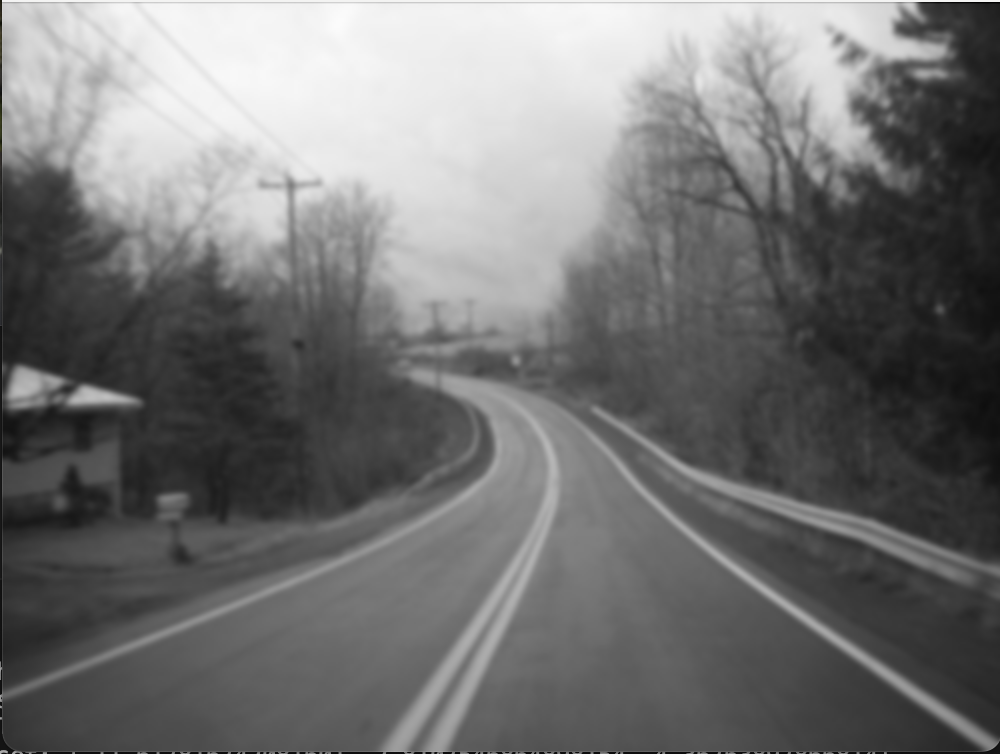
\includegraphics[width=0.7\textwidth]{3.png}     %圖片檔案名稱
    \caption{經高斯模糊處理之圖片}    %圖片檔案名稱
    \label{fig:3}    %為圖片添加標籤
    %如\ref{fig:2}所示
\end{figure}
%==============================內文==============================
\subsubsection{二值化}
%==============================內文==============================
\hspace{2em}將影像轉換為二值圖像,即只保留黑白兩種顏色,這有助於強調出車道線等重要特徵,便於後續的分析與處理。
固定閾值法:設定一個固定的閾值 $T$,當像素強度高於 $T$ 時設為白色,否則設為黑色。固定閾值法的公式如下。

\begin{align}
    I_{bin}(x,y) = 
    \begin{cases}
        1, & I(x,y) > T \\
        0, & I(x,y) \leq T
    \end{cases}
\end{align}

\begin{figure}[H]
    \centering
    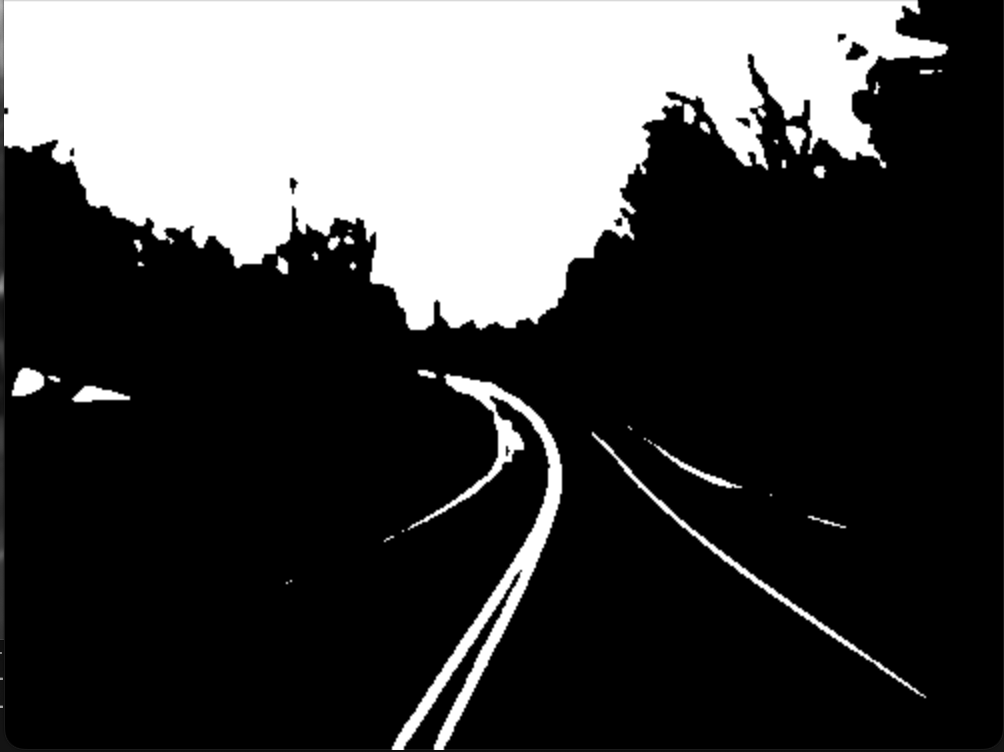
\includegraphics[width=0.7\textwidth]{4.png}     %圖片檔案名稱
    \caption{經二值化處理之圖片}    %圖片檔案名稱
    \label{fig:4}    %為圖片添加標籤
    %如\ref{fig:2}所示
\end{figure}

%==============================內文==============================

\subsubsection{Canny 邊緣偵測}
%==============================內文==============================
\hspace{2em}使用 Canny 邊緣偵測算子來提取影像中的邊緣信息,這有助於識別出車道的邊界或其他障礙物,為自走車的導航提供關鍵信息。
\begin{figure}[H]
    \centering
    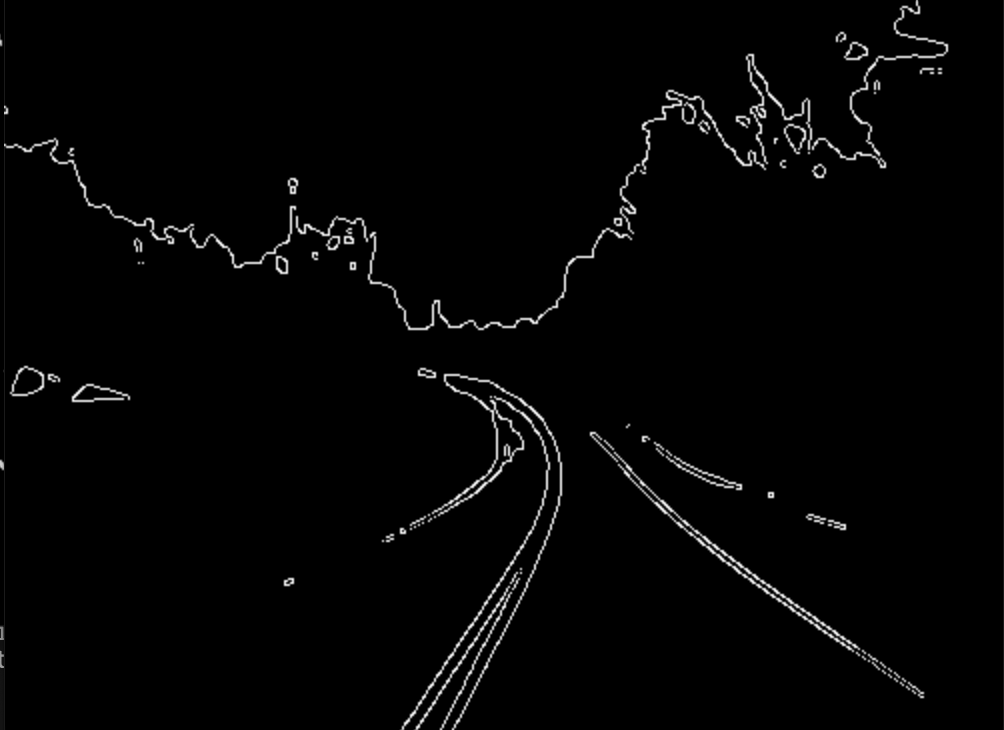
\includegraphics[width=0.7\textwidth]{5.png}     %圖片檔案名稱
    \caption{經邊緣偵測之圖片}    %圖片檔案名稱
    \label{fig:5}    %為圖片添加標籤
    %如\ref{fig:2}所示
\end{figure}
%==============================內文==============================

\subsection{偵測} 
%==============================內文==============================
\hspace{2em}圖像經過預處理後,接下來的步驟是偵測車道標線,並計算車輛的偏移量與偏移角度。
透過適當的演算法,能夠從二值化影像或邊緣偵測結果中提取關鍵特徵,並進一步分析車輛的行進狀態,以利於後續控制。
%==============================內文==============================

\subsubsection{掃描特定區域像素}
%==============================內文==============================
\hspace{2em}將首先,從影像中掃描特定的區域,通過檢測這些區域的像素值來獲取相關的幾何特徵。
在偵測車道標線時,並非整張影像都具有相同的重要性,因此可以選擇關鍵區域進行分析。例如,車輛前方的道路中央區域可能包含主要的行駛標線,而影像上方區域則可能包含過多的背景資訊,對偵測無實質幫助。
將使用滑動視窗法,使用固定大小的窗口在影像中移動,對每個區域進行局部分析,以提取潛在的車道標線位置。
\begin{figure}[H]
    \centering
    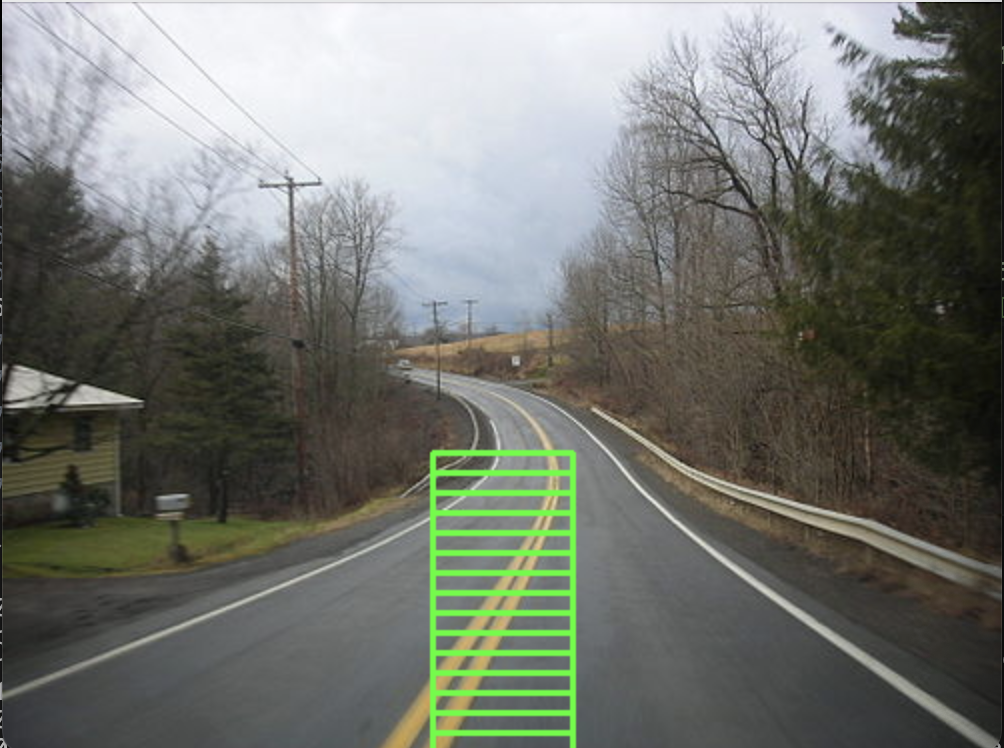
\includegraphics[width=0.7\textwidth]{6.png}     %圖片檔案名稱
    \caption{尚未滑動之視窗}    %圖片檔案名稱
    \label{fig:6}    %為圖片添加標籤
    %如\ref{fig:2}所示
\end{figure}
\begin{figure}[H]
    \centering
    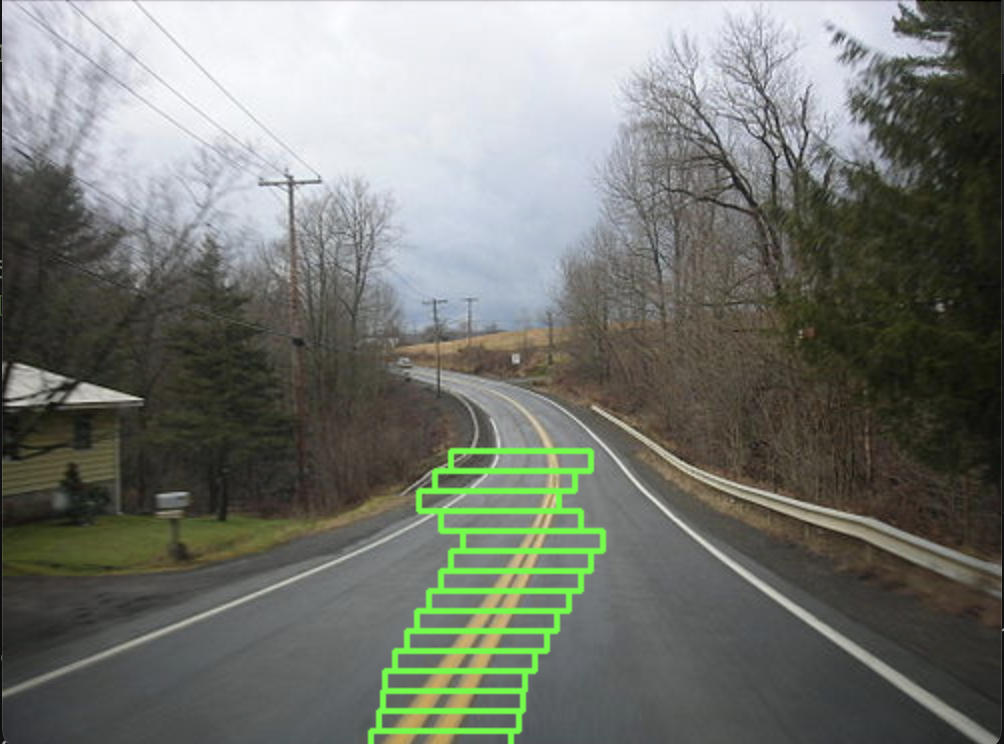
\includegraphics[width=0.7\textwidth]{7.png}     %圖片檔案名稱
    \caption{滑動後視窗}    %圖片檔案名稱
    \label{fig:7}    %為圖片添加標籤
    %如\ref{fig:2}所示
\end{figure}
%==============================內文==============================

\subsubsection{擬合曲線}
%==============================內文==============================
\hspace{2em}根據掃描到的像素資料,使用多項式擬合來擬合出車道線或相關物體的曲線,這樣可以準確地描述其形狀。

當獲取到標線像素點後,下一步是利用數學模型來擬合標線的形狀。由於車道標線通常具有一定的連續性與平滑度,可以使用 多項式擬合(Polynomial Fitting) 來描述其形狀。

\hspace{2em}對於普通道路,車道標線通常可以近似為二次曲線: \begin{align} y = ax^2 + bx + c \end{align} 其中,
$a,b,c$ 為待求的係數。使用最小二乘法(Least Squares Method, LSM) 來找到最適合這些數據點的曲線。

處理後如下圖所示,即可計算車輛的偏移量與偏移角度。
\begin{figure}[H]
    \centering
    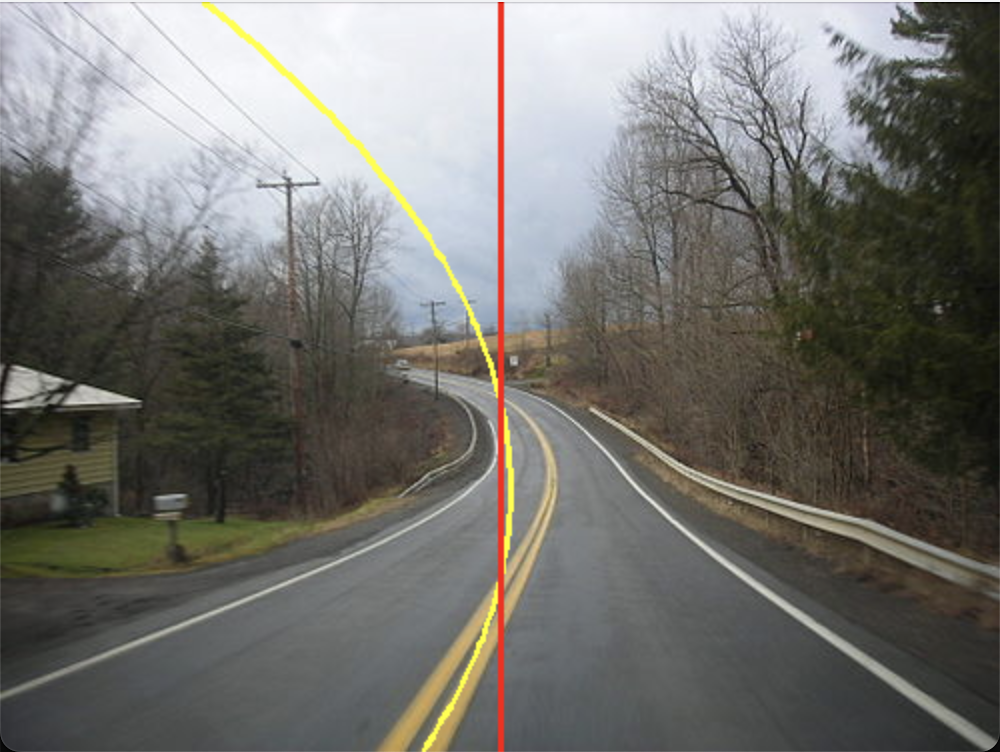
\includegraphics[width=0.7\textwidth]{8.png}     %圖片檔案名稱
    \caption{擬合後曲線與車輛行駛方向比較}    %圖片檔案名稱
    \label{fig:8}    %為圖片添加標籤
    %如\ref{fig:2}所示
\end{figure}
%==============================內文==============================

\subsubsection{計算偏移量、偏移角度}
%==============================內文==============================
\hspace{2em}根據擬合的曲線,計算出車輛當前的偏移量(與目標軌跡的水平距離)和偏移角度(與車道或目標方向的夾角)。這些數據將作為車輛調整行駛路徑的依據。

%==============================內文==============================

\subsection{控制} 
%==============================內文==============================
\hspace{2em}控制這一步分將使用模糊邏輯來實現全向輪之控制。

首先定義輸入變數與輸出變數。輸入變數為偏差角度$\theta$即位置偏移量$p$。輸入變數為前進速度$V_{x}$、側向數度$V_{y}$與角速度$\omega$ 。

隸屬函數將使用三角形隸屬函數(Triangular Membership Function, Trimf)。

模糊規則設計如下表(如表\ref{tab:fu1}、表\ref{tab:fu2}、表\ref{tab:fu3}所示),前進速度分為S(Slow, 慢速)、M(Medium, 中速)、F(Fast, 快速)。
側向速度分為LL(Leftmost, 最左)、L(Left, 左)、Z(Zero, 中間)、R(Right, 右)、RR(Rightmost, 最右)。
角速度分為CCW2(Counterclockwise 2, 強烈逆時針)、CCW(Counterclockwise, 輕微逆時針)、Z(Zero, 無旋轉)、CW(Clockwise, 輕微順時針)、CW2(Clockwise 2, 強烈順時針)。
\begin{table}[H]
    \centering
    \caption{$V_{x}$控制規則表}
    \vspace{6pt} % 增加空格
    \begin{tabular}{|c|c|c|c|c|c|}
    \hline
    \diagbox{\textbf{Angle($^\circ$)}}{\textbf{Position(cm)}} & \textbf{BL} & \textbf{SL} & \textbf{Z} & \textbf{SR} & \textbf{BR} \\
    \hline
    \textbf{BL} & S & S & M & S & S \\
    \hline
    \textbf{SL} & S & M & F & M & S \\
    \hline
    \textbf{Z} & M & F & F & F & M \\
    \hline
    \textbf{SR} & S & M & F & M & S \\
    \hline
    \textbf{BR} & S & S & M & S & S \\
    \hline
    \end{tabular}
    \label{tab:fu1}
\end{table}

\begin{table}[H]
    \centering
    \caption{$V_{y}$控制規則表}
    \vspace{6pt} % 增加空格
    \begin{tabular}{|c|c|c|c|c|c|}
    \hline
    \diagbox{\textbf{Angle($^\circ$)}}{\textbf{Position(cm)}}& \textbf{BL} & \textbf{SL} & \textbf{Z} & \textbf{SR} & \textbf{BR} \\
    \hline
    \textbf{BL} & RR & R & Z & L & LL \\
    \hline
    \textbf{SL} & RR & R & Z & L & LL \\
    \hline
    \textbf{Z} & RR & R & Z & L & LL \\
    \hline
    \textbf{SR} & RR & R & Z & L & LL \\
    \hline
    \textbf{BR} & RR & R & Z & L & LL \\
    \hline
    \end{tabular}
    \label{tab:fu2}
\end{table}

\begin{table}[H]
    \centering
    \caption{$\omega$控制規則表}
    \vspace{6pt} % 增加空格
    \begin{tabular}{|c|c|c|c|c|c|}
    \hline
    \diagbox{\textbf{Angle($^\circ$)}}{\textbf{Position(cm)}}& \textbf{BL} & \textbf{SL} & \textbf{Z} & \textbf{SR} & \textbf{BR} \\
    \hline
    \textbf{BL} & CW2 & CW2 & CW2 & CW2 & CW2 \\
    \hline
    \textbf{SL} & CW & CW & CW & CW & CW \\
    \hline
    \textbf{Z} & Z & Z & Z & Z & Z \\
    \hline
    \textbf{SR} & CCW & CCW & CCW & CCW & CCW2 \\
    \hline
    \textbf{BR} & CCW2 & CCW2 & CCW2 & CCW2 & CCW2 \\
    \hline
    \end{tabular}
    \label{tab:fu3}
\end{table}

最後進行模糊推理與去模糊化,給定輸入 $\theta_{\text{in}}$ 和 $p_{\text{in}}$,計算它們在模糊集合中的的隸屬度:
\begin{align}
    \mu_A(\theta_{\text{in}}), \quad \mu_B(p_{\text{in}})\label{eq:1}
    %式label{eq:2}
\end{align}
然後對於每個模糊規則$R_i$,使用最小推理法(Mamdani推理法)計算輸出的強度:
\begin{align}
    \mu_{\text{rule}} = \min(\mu_A, \mu_B)\label{eq:2}
    %式label{eq:2}
\end{align}
最後,使用重心法(Centroid Method)計算輸出,其中 $y_i$ 是輸出變數的取值,$\mu_i$ 是對應的隸屬度。
\begin{align}
    y^* = \frac{\sum \mu_i y_i}{\sum \mu_i}\label{eq:3}
    %式label{eq:2}
\end{align}

即可得到了模糊控制輸出的 $V_x$, $V_y$, $\omega$。已知麥克納姆輪的速度模型如下,可得知每一顆輪子之速度,即可換算成輪子所需轉速。

\begin{align}
    \begin{bmatrix}
        V_{FL} \\
        V_{FR} \\
        V_{RL} \\
        V_{RR}
        \end{bmatrix}
        =
        \begin{bmatrix}
        1 & -1 & -1 & 1 \\
        1 & 1 & 1 & 1 \\
        -1 & 1 & -1 & 1 \\
        1 & -1 & 1 & -1
        \end{bmatrix}
        \begin{bmatrix}
        V_x \\
        V_y \\
        \omega
        \end{bmatrix}
\end{align}
%==============================內文==============================

\section{\centering 人機界面的功能概述}

%==============================內文==============================
\hspace{2em}人機界面將主要提供使用者監控控自走車,顯示車輛的實時影像及運行狀態(如行駛速度、偏差角度等)。
顯示車輛是否正確沿著標線行駛,若有偏離,顯示偏離的程度。

\section{\centering 研究進度與預估花費}


\begin{table}[H]
    \centering
    \caption{預估花費}
    \vspace{6pt} % 增加空格
    \label{tab:money}
    \begin{tabular}{ll}
        \toprule
        \textbf{項目} & \textbf{花費(元)} \\
        \midrule
        esp32-cam & 330  \\
        Wemos D1   & 200  \\
        tt減速馬達 & 50*4  \\
        \bottomrule
    \end{tabular}
\end{table}


\begin{center} % 使甘特圖居中

    \vspace{6pt} % 增加空格

    \begin{ganttchart}[
        x unit=1.2cm, % 設定 X 軸單位長度
        y unit chart=0.5cm, % 設定 Y 軸單位長度
        vgrid, % 垂直網格線
        hgrid, % 水平網格線
      ]{5}{16} % 甘特圖時間範圍(第5週到第16週)
      
      \gantttitlelist{5,6,7,8,9,10,11,12,13,14,15,16}{1} \\ % 時間軸
      
      \ganttbar{程式撰寫}{5}{6} \\ % 第一個任務
      \ganttbar{材料購買}{6}{9}\\
      \ganttbar{影像傳輸}{7}{10}\\
      \ganttbar{命令傳輸}{9}{11}\\
      \ganttbar{參數調整}{10}{14}\\
      \ganttbar{報告撰寫}{13}{15}\\
    \end{ganttchart}
        \begin{figure}[H]
            \caption{研究計畫甘特圖}
        \end{figure}
\end{center}
    







    
    







%==============================內文==============================


\section{\centering 參考文獻}
\vspace{-3.5em}  % 減少與上方內容的間距
\renewcommand{\refname}{}  % 去除 "References" 標題
\printbibliography  % 列出參考文獻

\end{document}

%=============================================================================================================================
%=============================================================================================================================
%=============================================================================================================================


\begin{comment}

\section{\centering 緒論}
\subsection{研究問題} 
\subsubsection{違規車輛偵測}
    
    %==============================圖片==============================
\begin{figure}[H]
    \centering
    \includegraphics[width=0.7\textwidth]{截圖 2025-01-24 03.21.17.jpg}     %圖片檔案名稱
    \caption{這是圖片的標題}    %圖片檔案名稱
    \label{fig:example2}    %為圖片添加標籤
    %如\ref{fig:example1}所示
\end{figure}
    
    %==============================數學公式==============================
\begin{align}
    a &= b + c \label{eq:1}
    \\
    d &= e - f \label{eq:2}
    %式label{eq:2}
\end{align}
    
    %==============================表格==============================
\begin{table}[H]
    \centering
    \caption{C922 Pro Stream 規格}
    \vspace{6pt} % 增加空格
    \label{tab:C922 Pro}
    \begin{tabular}{ll}
        \toprule
        \textbf{項目} & \textbf{規格} \\
        \midrule
        解析度  & 1280$\times$720 (HD) \\
        幀率  & 30fps \\
        水平視角 & 70.42$^\circ$ \\
        垂直視角  & 43.3$^\circ$ \\
        \bottomrule
    \end{tabular}
\end{table}
    
    \end{comment}
        